\documentclass[hyperref={bookmarks=false},aspectratio=169]{beamer}
\usepackage[utf8]{inputenc}

\usepackage{datetime}
\newdateformat{monthyeardate}{\monthname[\THEMONTH] \THEYEAR}
% ---------------  Define theme and color scheme  -----------------
\usetheme[minimal]{Iist}  % 3 options: minimal, sidebarleft, sidebarright

%\setbeamertemplate{footline}[frame number]

% ------------  Information on the title page  --------------------
\title[]
{Presentation Title}

\subtitle{Subtitle if any}

\author[]
{Author 1\inst{1} \and Author 2\inst{1}}

\institute[Caltech]
{
  \inst{1}
  Department of Aerospace Engineering\\
  Indian Institute of Space Science and Technology\\\vspace{0.2cm}
  
\includegraphics[width=1.2cm]{./figures/iist_logo.png}
  %\and
  %\inst{2}
  %Department of Aerospace Engineering\\
  %Indian Institute of Space Science and Technology
}

\date[\today]
{Structural Dynamics and Vibration Lab - IIST\\ \monthyeardate\today}
%------------------------------------------------------------

%------------------------------------------------------------
%The next block of commands puts the table of contents at the 
%beginning of each section and highlights the current section:

\AtBeginSection[]
{
  \begin{frame}
    \frametitle{Table of Contents}
    \tableofcontents[currentsection]
  \end{frame}
}
%------------------------------------------------------------


\begin{document}
{
\setbeamertemplate{footline}{}
\frame{\titlepage}  % Creates title page
}
%---------   table of contents after title page  ------------
 
\begin{frame}
\frametitle{Table of Contents}
\tableofcontents
\end{frame}

%---------------------------------------------------------


\section{Topic 1}

%---------------------------------------------------------
%Changing visivility of the text
\begin{frame}
\frametitle{IIST WIKI}
Indian Institute of Space Science and Technology (IIST) is a government-aided institute and deemed university for the study and research of space science, located at Valiamala, Nedumangad, Thiruvananthapuram, Kerala. 

\begin{itemize}
    \item<1-> Conscientia is the Annual Astronomy and Technology Festival of IIST.[23] Conscientia offers various challenging events in different fields of engineering and science, including astronomy, aerospace engineering, electronics, computer science, mechanical engineering, robotics, etc. 
    \item<2-> Dhanak is the Annual Cultural Festival of IIST. 
    \item<3-> Started as an intra-college event in March 2012, IIST MUN has now become a national inter-college Model United Nations with United Nations General Assembly council held successfully in September\textbf{ 2012, 2013}, October 2014 and April 2015.
\end{itemize}

\end{frame}

%---------------------------------------------------------


%---------------------------------------------------------
%\begin{frame}  % Example of the \pause command
%This slide is to test mathematical formulas \pause
%
%$$E=mc^2$$ \pause
%
%as well as the ``pause'' functionality
%\end{frame}
%---------------------------------------------------------

\section{Topic 2}

%---------------------------------------------------------
%Highlighting text
\begin{frame}
\frametitle{Topic 2 }

IIST has signed a number of memorandums of understanding (MoUs) with international universities and Institutions for joint research, and exchange of  \alert{students and faculty.}.

\begin{block}{Definition}
IIST has signed a number of memorandums of understanding (MoUs) with international universities and Institutions for joint research, and exchange of  \alert{students and faculty.}.
\end{block}


\end{frame}
%---------------------------------------------------------


%---------------------------------------------------------
%Two columns
\begin{frame}
\frametitle{Campus}

\begin{columns}

\column{0.45\textwidth}

\begin{figure}
    \centering
    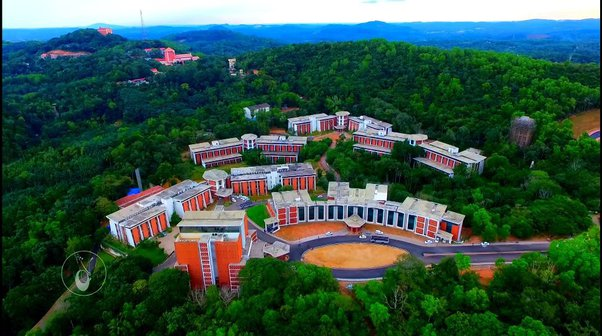
\includegraphics[width=\columnwidth]{./figures/iist}
    \caption{IIST- Aerial view}
    \label{fig:hollywood_prank}
\end{figure}


\column{0.55\textwidth}
At its inception, the institute started functioning at the ATF Campus, under Vikram Sarabhai Space Centre, Thiruvananthapuram (Trivandrum), Kerala. Modern environmentally friendly buildings of unique architecture merge well with the thickly wooded campus of 100 acres situated on the foothills of Sahyadri.

\small{(Reference: http://www.iist.ac.in)}\\
To cite an article/ book/ proceedings


\end{columns}
\cite{santhosh2021generalized} second reference: \cite{ROMANO201714} Third reference:\cite{ROMANO2017151} Fourth reference: \cite{Strogatz1991} Fifth Reference: \cite{strogatz2004sync} Sixth Reference:\cite{thomson1996theory}
\end{frame}
%---------------------------------------------------------

\section{References}
\begin{frame}[allowframebreaks]{References}

	%\tiny  % uncomment tiny if you need to include more number of references in a frame.
	\bibliographystyle{apalike}
	\bibliography{reference.bib}
	
\end{frame}


\end{document}
